\documentclass[12pt]{report}                 % hauteur des fontes (11 ou 12 pt), on peut ajouter d'autres options
                                             % on indique aussi le type de document (paper, report, thesis, ...)
% Ajout des packages : il en existe de très nombreux. 
% la liste ici est assez minimaliste.

% IL EST CONSEILLE D'APPELER LE FICHIER PRINCIPAL "main.tex" ou bien un nom très simple explicite (ici report.tex)

\usepackage[english]{babel}                  % choix ce la langue
%
%  choix de la fonte:
%\usepackage{times}
\usepackage{palatino}
% sinon fonte par défaut
\usepackage[T1]{fontenc}

\usepackage{setspace}                           % gestion de l'interligne%\usepackage{floatflt,fancyheadings}
\usepackage{fancyhdr}                           % présentation de la page (bas , haut, numéros, etc ...)
\usepackage{amssymb,amsmath}                    % symbôles mathématiques 
\usepackage{empheq}                             % complément à amsmath pour améliorer les équations (subequations)
\usepackage{float}                              % Positionnement des figures
\usepackage{graphicx,caption}                   % fogures, graphiques, légendes
%\usepackage{psfig,epsfig,epsf}                 % pour gérer les fichiers postscript (éviter de les utiliser)
\usepackage{color}                              % gestion des couleurs, attention, interférences avec package xcolor
\usepackage{mdframed}                           % pour faire de jolies encadrements
\usepackage[most]{tcolorbox}                    % Pour ajouter de la couleur dans les encadrements
\usepackage{makecell}                           % Pour améliorer le rendu des tableaux

\bibliographystyle{acm}                         % gestion du rendu de la bibliographie. Peut être mis dans le corps du fichier

% gestion de la géométrie de page, en pouces et mm
\hoffset=-1in                                   % décalage horizontal
\voffset=-1.5in                                 % décalage vertical
\topmargin=15mm                                 % marge supérieure 
\headheight=5mm                         
\headsep=15mm
\textheight=240mm                               % taille de la page où on peut écrire
\oddsidemargin=15mm                             % marge des pages impaires
\evensidemargin=15mm                            % marge des pages paires
\textwidth=180mm                                % largeur de la page où on peut écrire 
\pagestyle{headings}                            % style de la page (cf fancyhdr)


%    COMMANDES GENERALES PERSONNELLES

\renewcommand{\textfraction}{.10}
% mathématiques:
\newcommand{\derp}[2]{ \frac{ \partial #1 }{ \partial #2}}
\newcommand{\der}[2]{ \frac{ d #1 }{ d #2}}
\newcommand{\dsp}{\displaystyle}
\newcommand{\bs}[1]{\boldsymbol{#1}}
\newcommand{\degree}{\ensuremath{^\circ}}
% tailles de fontes
\newcommand{\sr}{\scriptsize}
\newcommand{\st}{\tiny}
% style et espacements
\newcommand{\itemb}{\item [$\bullet$]}
\newcommand{\vs}[1]{\vspace{ #1 cm}}
\newcommand{\hs}[1]{\hspace{ #1 cm}}
% couleurs
\newcommand{\rouge}[1]{\textcolor{red}{ \it  #1}}
\newcommand{\bleu}[1]{\textcolor{blue}{ \it  #1}}
\newcommand{\gris}[1]{\textcolor{gray}{ \it  #1}}
\newcommand{\red}[1]{\textcolor{red}{#1}}
\newcommand{\alert}[1]{\textcolor{red}{ \bf  #1}}   % en référence à Beamer, pour mettre en valeur


% Cadres colorés avec messages:
\newcommand{\todo}[1]{\tcbset{colback=red!5!white,colframe=red!85!black,
code={},
fonttitle=\bfseries}
\begin{tcolorbox}[code={},
title= To do]
#1
\end{tcolorbox}
}
\newcommand{\Note}[1]{\tcbset{colback=red!5!white,colframe=green!65!black,
code={},
fonttitle=\bfseries}
\begin{tcolorbox}[code={},
title= Note]
#1
\end{tcolorbox}
}
\newcommand{\Attention}[1]{\tcbset{colback=red!30!white,colframe=blue!50!red,
code={},
fonttitle=\bfseries}
\begin{tcolorbox}[code={},
title= Attention]
#1
\end{tcolorbox}
}
\newcommand{\Important}[1]{\tcbset{colback=red!10!white,colframe=blue!50!red,
code={},
fonttitle=\bfseries}
\begin{tcolorbox}[code={},
title= Important]
#1
\end{tcolorbox}
}
\newcommand{\Def}[2]{\tcbset{colback=blue!10!white,colframe=green!70!white,coltitle=black,
code={},
fonttitle=\bfseries}
\begin{tcolorbox}[code={},
title= Definition : #1]
#2
\end{tcolorbox}
}
\newtcbox{\mymath}[1][]{%
    nobeforeafter, math upper, tcbox raise base,
    enhanced, colframe=blue!30!black,
    colback=blue!30, boxrule=1pt,
    #1}

% Dossiers par défaut contenant les figures (TRES IMPORTANT)
\graphicspath{{Figures/},} 


%%%%%%%%%%%%%%%%%%%%%%%%%%%%%%%%%%%%%%%%%%%%%%%%%%%%%%%%%%%%%%%%%%%%%%%%%%%%%%%
%
%                    DEBUT DU DOCUMENT
%
%%%%%%%%%%%%%%%%%%%%%%%%%%%%%%%%%%%%%%%%%%%%%%%%%%%%%%%%%%%%%%%%%%%%%%%%%%%%%%%

\begin{document}

% créer une page spécifique pour le titre
\begin{titlepage}

\begin{center}
{
\large \textbf{ Universit\'e Paul Sabatier, Toulouse  }

\vspace{0.5cm}

\begin{figure}[h] 
    \begin{center}
    
\includegraphics[width=0.1\textwidth]{Figures/Uni.png}
    \hspace{3cm}
    
\includegraphics[width=0.2\textwidth]{Figures/IMFT_Logo.pdf}
    \end{center}
\end{figure} 

\vspace{0.5cm}

\textbf{Institut de M\'ecanique des Fluides de Toulouse}

\vspace{1cm}

\Huge \textbf{\'Ecrire un rapport}

\vspace{0.5cm}
\Large
Obtenir une compétence transversale durant ces études supérieures.

}

\vspace{0.5cm}

\textbf{Christophe  Airiau }

\vspace{1cm}

Christophe.Airiau@imft.fr

\vspace{0.5cm}

\today


\begin{figure}[h] 
    \begin{center}
    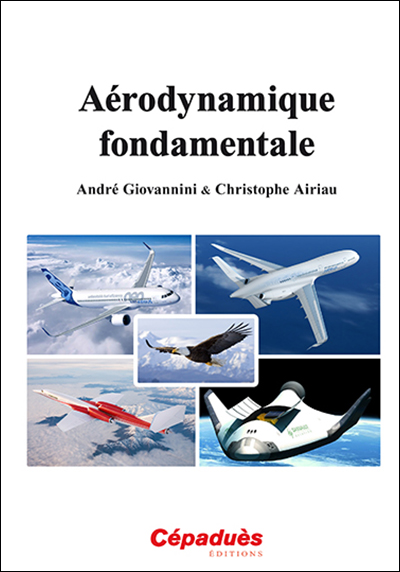
\includegraphics[width=0.2\textwidth]{Figures/Livre1.jpg}
    \hspace{3cm} 
    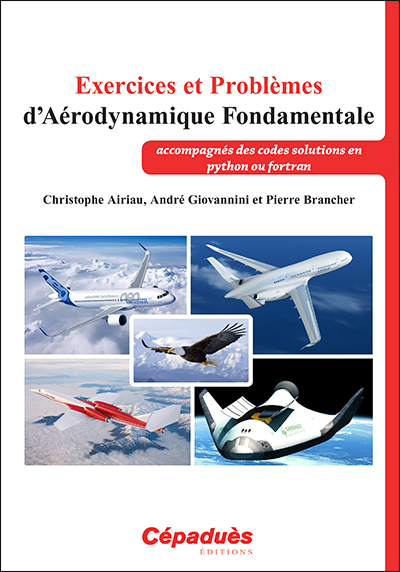
\includegraphics[width=0.2\textwidth]{Figures/Livre2.jpg}
    \end{center}
\end{figure} 

{\scriptsize 
\setstretch{0.4}
\begin{itemize}
\item \rouge{Ne pas hésiter à ajouter de jolies figures ou photos en page de titre, en lien avec le rapport}
\item \rouge{mettre les logos et le nom de l'organisme d'accueil}
\item \rouge{mettre une date avec éventuellement la mention provisoire, ou la version}
\item Titre expressif en gras, éventuellement ajouter un sous-titre, nom des auteurs et affiliation
\item \rouge{Ajouter le nom des encadrants avec affiliation}
\item Mise en forme: choix personnel ou imposé par le commanditaire ou organisme d'accueil
\end{itemize}
}
\end{center}
\end{titlepage}

\cleardoublepage  
\pagenumbering{roman}   % numérotation des pages avant l'introduction

\setcounter{page}{1}
\setcounter{secnumdepth}{3}        
\setcounter{tocdepth}{4}       % pour définir la profondeur du sommaire  

% Tables des matières, ajouter le nom en haut de la page
\markboth{{Table des mati\`eres}}{}
\markright{{Table des mati\`eres}}
\tableofcontents
% 
\cleardoublepage

% ajout des noms du chapitre en haut de page
\renewcommand{\chaptermark}[1]{\markboth{{\thechapter.\ #1}}{}}
\renewcommand{\sectionmark}[1]{\markright{{\thesection.\ #1}}}

% ajout du résumé (recommandé en français et anglais)
\addcontentsline{toc}{chapter}{Résumé}
%*******************
\section*{Résumé}
%*******************
%% résumé


\setstretch{1.5}

Le résumé se trouve possiblement à trois endroits:
\begin{enumerate}
	\item  juste après la page titre
	\item  sur la dernière page
	\item  sur la quatrième page de garde (dos de la couverture du rapport)
\end{enumerate}


Il est très souvent écrit en anglais et accompagné de \textbf{cing mots clés}
qui permettent ensuite un indexage plus facile dans les bibliothèques ou sur internet.

Le résumé  est écrit très souvent en anglais, et 
peut être  accompagné d'une version française.

Un résumé ne dépasse jamais une page, soit de 15 à 20 lignes environ.

Enfin on peut choisir une taille de fonte légèrement plus petite que celle
du document, ce qui permet d'allonger le texte ou de mettre les deux versions
anglaise et française sur une seule page.


Le résumé rappelle les éléments suivants:

\begin{itemize}
\item le contexte, la motivation et les objectifs du projet
\item les méthodologies adoptées pour résoudre le problème posé
\item le ou les principaux résultats originaux incluant les analyses
\item la ou les principales conclusions
\item une perspective intéressante
\end{itemize}


\setstretch{1.}
 

% ajout d'une nomenclature (optionnel)
\addcontentsline{toc}{chapter}{Nomenclature}
%***********************
\chapter*{Nomenclature}
%**********************
% Nomenclature

La nomenclature sera discutée dans la section \ref{sec:nomenclature}



\begin{center}
\begin{tabular}{p{4.cm} p{12cm}l}
 \Xhline{2pt}
  Name, Notations   &  Meaning  \\  \Xhline{1pt}
  C0, C1, ...       &  A given general geometrical configuration \\
  H0, H1, ...       &  HTT configuration baseline \\
  \hline
  \textbf{Acronym}  &                             \\
  CFD               & Computational Fluid Dynamics \\
  DNS               & Direct Numerical Simulation \\
  \hline
  \textbf{Nondimensional number} &  \\
  $Re$              & Reynolds number  \\
  $Ma$               & Mach number    \\
  $Pr$              & Prandtl number \\       
  \hline
  \textbf{Physical quantity} &    \\
  $\rho$           	& Gas density [$\rm kg/m^3$] \\
  $\mu$             & Dynamic viscosity [$\rm kg.m^{-1}.s^{-1}$]\\
  $T$               & Temperature [$\rm K$] \\
  $\Delta T$        & Temperature variation \\
  $p$               & Pressure [$\rm Pa$]\\
  $L$               & Length (of the body) [$\rm m$]  \\
  $x,y, z$          & Cartesian coordinates \\
  $\textbf{r}=[r_i]$      & Position vector\\
  $\Delta t$        & Time step [$\rm s$] \\
  $q$               & heat conduction flux density [$\rm W/m^2$] \\
   \Xhline{1pt} 
  \textbf{superscript}        &  \\
  *               & Physical quantity   \\
  t               & Transposition \\
  \hline
  \textbf{subscript}            &  \\
  gas                & refered to a gas \\
  wall               & refered to a wall value \\
 \Xhline{2pt}
\end{tabular}
 \end{center}


 
\cleardoublepage

% ajout d'une liste des figures (optionnel)
\listoffigures
\cleardoublepage

% ajout d'une liste des tableaux (optionnel)
\listoftables
\cleardoublepage

% Numérotation des pages en chiffres classiques,réinitialisaiton à 1.
\renewcommand{\thepage}{\arabic{page}}
\setcounter{page}{1} 

% On ajoute maintenant les sections oo les chapitres,
% dans des fichiers spécifiques. Plus facile à gérer.

% ********************************
\chapter{Introduction}
% *******************************
% Chapter introduction
\label{sec:introduction}
% **********************************
\section{Introduction}
% **********************************

Dans la vie d'un étudiant et d'un professionnel, on doit rédiger des rapports. \`A l'université on considère
par défaut que l'étudiant doit apprendre par lui-même à faire celà en cherchant des exemples. Dans des universités
étrangères cela fait partie d'un enseignement. 

On peut s'apercevoir que au final, après 5 années d'études, peu savent préparer et rédiger un beau rapport ou un beau compte-rendu
d'un travail donné.

Il m'a semblé donc important de préparer un document assez complet, mais pas exhausitif rappelant les points essentiels,
distribuables à tous les niveaux de la licence au master. 

Ce document est rédigé sur la base de mon expérience dans l'écriture de cours,
 de livres, d'articles, de rapports techniques.
 Il prend aussi en compte  l'expérience acquise par des expertises très nombreuses de projets scientifiques ou d'articles pour des revues internationales.

Enfin, mon expérience a été renforcée  au cours de ma carrière par la lecture  de centaines de rapports
de stage ou de projets, et un grand nombre de thèses de doctorat.

Enfin la lecture d'ouvrage de référence sur l'écriture de rapports joints dans la bibliographie a permis de compléter l'ensemble.
 
Ce rapport en latex pourra servir d'exemple (templates) modifiable, mais les conseils donnés sont aisément transposables, 
parfois même plus facilement dans d'autres types de logiciels comme MS Word ou OO Writer.
Bien que  Latex présente des facilités  bien pratiques à l'écriture de rapport il n'est pas préféré au sein du monde industriel
qui favorise largement MS Word. Rappelons que Latex est un logiciel libre et 
donc privilégié à l'université et dans le monde de la recherche.
 
Enfin pour clore cette section il faut préciser qu'on ne perd par plus de temps à faire bien les choses que de mal les faire.
Même souvent c'est le contraire, car bien faire les choses amènent des questions utiles pour améliorer le contenu.


% ********************************
\section{Compétences à acquérir}
% *******************************

La vocation des Masters est de fournir aux étudiants des connaissances scientifiques et techniques et des compétences 
dans le but de favoriser au mieux une future insertion professionnelle.
 On peut y ajouter l'introduction des méthodologies de travail, des méthodes de pensées qui permettront d'aider à une
 formation tout au long de la vie, en autonomie ou pas. 

Il existe suivant les domaines scientifiques, d'ingénierie, de professions visées, 
 un grand nombre de compétences à acquérir tout au long des études dans l'enseignement supérieure, 
avec des niveaux  de difficultés progressifs.

Une des plus importantes  compétences transversales,  commune  consiste à 
 savoir rédiger correctement un rapport de qualité  qui est un document écrit en général archivé et donc transmissible.

Le rapport est une trace, voir un signature de l'auteur qu'il laisse derrière lui,
et qui met en avant ses compétences ou parfois son manque de compétence. 

Les exigences en termes de qualité et de rendu ont augmenté progressivement au cours des années,
 notamment à cause de l'arrivée d'outils informatiques très performants pour l'aide à l'écriture et à la publication.

Il convient donc se de former, et d'apprendre en autonomie à rédiger un document de qualité. 

Des recherches sur internet montrent que finalement on trouve très peu de documents qui indiquent clairement 
aux étudiants comment rédiger un compte rendu de TP ou un rapport de stage ou de projet. 
 

Un premier document a été rédigé  sur l'écriture d'un compte-rendu de TP.
Je continue  cette démarche en proposant ce document sur la rédaction d'un rapport de projet ou de stage.

Les documents ne sont pas parfaits et finalement présentent mon point de vue personnel.
Certaines parties peuvent notamment être plus tournées vers la science ou l'ingénierie, et ne conviendront pas naturellement 
à des rapports
dans d'autres domaines comme la santé,  les sciences humaines, les sciences économiques ou le droit.

J'espère  que ce document sera partagé, et que par des retours pourront  participer à son amélioration.


On peut conclure cette section en rappelant quelques compétences à acquérir pour rédiger un rapport de qualité, au moins dans la forme:

\begin{itemize}
\item être capable de maîtriser un ou plusieurs  logiciels de publication (MS Word, OO Write, Latex). Cela inclus:
	\begin{itemize}
	\item le choix ou la définition d'un style global
	\item l'ajout de tableaux ou de figures avec numérotation et titre
	\item la gestion de haut et bas de page
	\item la gestion d'une bibliographie avec référencement automatique, associée  à une  base de donnée bibliographique
	\item la gestion de la mise en page (figures et tableau à la bonne position par exemple)
	\end{itemize} 
\item être capable d'utiliser (voir de maîtriser) des outils de traitement d'images (GIMP par exemple) et des outils de dessin vectoriel (INKSCAPE par exemple).
       Des exemples sont données par la suite.
\item être capable de rédiger dans un français correct (ou un anglais correct) 
\item être capable d'organiser ses réflexions, ses analyses pour produire un document structuré 
\item être en mesure d'utiliser les fonctions graphiques de logiciels ou de langage (Python, ...) afin de produire des figures de qualité
\item \alert{A COMPLETER} 
\end{itemize}



%**********************
\section{Les rapports}
%**********************

%****************************************
\subsection{Différents types de rapport}
%***************************************

Pour un étudiant on peut considérer trois types de rapports:
\begin{itemize}
\item un compte-rendu de TP  qui est un petit rapport sur une activité très contrôlée et très formatée par un énoncé relativement précis qui sert de guide.
En général le compte-rendu ne dépasse pas les 20 pages, et très souvent les 10 pages.
\item un rapport de projet, scientifique ou technique. C'est un rapport plus libre qui doit mettre en avant un travail en autonomie d'un étudiant. 
Sa longueur est entre 10 et 30 pages. 
\item un rapport de stage. Ce dernier est une version améliorée d'un rapport de projet. La durée d'un stage est de plusieurs mois. Pour cette durée
 on estime qu'une longueur d'une quarantaine de pages, hors annexes, est amplement suffisante.
\end{itemize}

La taille d'un rapport suivant son type  est rappelée dans le tableau \ref{table:report}. 
La dernière ligne du tableau donne un élément de réflexion sur sa structure primaire, et donc la  possibilité d'utiliser
 des chapitres qui ne sont pas nécessaires si le document contient trop peu de pages.

\begin{table}[htb]
\setstretch{1.2}
\small
\centering
\begin{tabular}{p{2cm} p{4.5cm} p{4.5cm} p{4.5cm}}
 \Xhline{2pt}
type &   comte-rendu de TP  & rapport de projet &  rapport de stage \\ \Xhline{1pt}
pages &  5 - 20              & 10 - 30          &  30 - 40 \\
Chapitre & Non               & Peut-être        & Probable \\  \Xhline{2pt}
\end{tabular}
\caption{Longueur de différents rapports et existence de chapitre.}
\label{table:report}
\end{table}

\textbf{Un certain nombre d'indications fournies dans le document sur la rédaction d'un compte-rendu de Travail Pratique\footnote{travail de laboratoire (labwork en anglais)} restent valables et sont reprises dans ce document.}


%*******************************************************
\subsection{Rapport scientifique ou rapport technique}
%*******************************************************

La différence majeure entre un rapport scientifique et un rapport technique 
se situe dans le contenu.
 Naturellement cela parfois se répercute  aussi sur la forme. 
 Un rapport scientifique est beaucoup plus difficile à écrire et souvent plus long qu'un rapport technique.

On va prendre un exemple classique dans le milieu de la recherche afin d'illustrer les différences fondamentales.

%*********************************
\subsubsection{Rapport technique}
%*********************************

Une entreprise contacte une équipe de recherche  pour mener des essais en soufflerie. 
On doit effectuer voir concevoir le montage,  les essais et rédiger un rapport technique.
Ce rapport décrit le montage, explique comment les essais ont été menés et fournit les résultats des essais 
ainsi que des statistiques permettant d'évaluer les erreurs de mesure.

Un rapport technique contient donc uniquement des données techniques, utilisables plus tard. 

On peut y trouver parfois un peu de traitement de données (i.e sur les résultats).

Il ne faut pas oublier cependant que certaines techniques ou objet technique 
font appel à beaucoup de sciences, et ainsi la description des moyens de mesure employés peuvent
demander des connaissances pointues. 


%*********************************
\subsubsection{Rapport scientifique}
%*********************************

Une entreprise contacte une équipe de rechercher 
pour mener une étude aérodynamique sur le décollement de la couche limite (l'écoulement) autour d'un profil d'aile, en utilisant en partie les moyens
expérimentaux à disposition, comme une soufflerie ou un canal hydrodynamique.

On effectue le montage et les essais.
 En plus de cela est fournie  une bibliographie sur la problématique qui requiert des connaissances scientifiques sur la problématique, et une capacité de synthèse.
  Ensuite  des calculs de couche limite ou des simulations numériques sont effectuées.
  Enfin on doit conduire un post-traitement des données expérimentales en les comparant aux résultats des simulations.
 \'Eventuellement des codes plus ou moins important devront être écrits.   
   Finalement on conclut ce travail en donnant des perspectives sur l'évolution du projet.

On voit ici qu'il y a eu un travail scientifique sérieux qui a été effectué et qui doit être rédigé.
Le rapport sera un rapport scientifique qui contiendra à la fois les aspects expérimentaux, la théorie, les simulations et toutes les analyses produites,
 avec une conclusion sur les aspects scientifiques du problème.

Un rapport scientifique peut se baser sur un rapport technique afin d'avoir des résultats de référence.


%**********************************
\subsection{Rapport de projet}
%*********************************

Dans l'industrie ou la recherche tout travail est lié à un projet
 et donc le rapport de projet est une synthèse  partielle ou complète 
 des actions menées dans le projet, concaténant des informations de rapports techniques et scientifiques éventuellement.
 Il peut être complété par des informations ou des parties traitant des aspects organisationnels et économiques.

\`A l'image de cela, un rapport de projet dans l'enseignement doit contenir un certain nombres d'informations assez similaires à celles d'un projet
scientifique ou industriel.

Une  thèse  de doctorat entre  dans cette catégorie.

Cela sera discuté dans le chapitre \ref{cha:structure}. 


%**********************************
\subsection{Rapport de stage}
%*********************************

Un rapport de stage est formaté comme un rapport de projet. Quelques différences notables sont à ajourer:
\begin{itemize}
\item La page des remerciements est obligatoire, il faut remercier l'entreprise et les collègues qui vous ont aidés
\item Il faut rajouter un chapitre ou une section de 2 à 4 pages qui décrit les activités de l'entreprise et la position du stagiaire au sein de l'entreprise
\item Les attendues du stage doivent être indiquées dans l'introduction
\item Il faut mettre en avant le travail effectué et les apports pour l'entreprise.
\item Il faut éviter, comme dans tous les rapports, un plagiat en reprenant des pages entières de rapport des stagiaires
 qui ont déjà travaillé sur une partie projet. Cela se voit facilement en général et donne une mauvaise impression au lecteur évaluateur.
\end{itemize}

% ************************************
\subsection{Evaluation d'un rapport}
% ************************************

Un document écrit est toujours évalué sur deux aspects:

\begin{itemize}
\item \textbf{la forme} qui correspond à des choix éditoriaux, de style, de mise en forme du texte, des images, des figures et des sections. 
Utiliser des items par exemple est un choix de style qui permet de mettre en évidence des points plus facilement.
\item \textbf{le fond} 
 qui  correspond au texte écrit, ou choix du contenu des figures,
  des tableaux et  des équations présentées.
  
  Le fond couvre tout ce qui dépend  du sujet du rapport.
\end{itemize}


On pourrait  penser a priori que les deux aspects sont totalement découplés et donc en négliger un par rapport à l'autre.
Dans la réalité, il est très rare d'avoir un bon fond quand la forme est très mauvaise. Quelqu'un qui a passé 
du temps à produire un beau document a aussi 
passé du temps à produire un travail scientifique de qualité.

Dans la suite de ce document on parlera uniquement de la forme. 
Le fond de ce document est de donner des lignes de conduite, des guides
afin d'écrire un rapport de qualité sur la forme.


%*****************************************
\section{Outils utilisés pour ce rapport}
%****************************************

Ce rapport a été écrit avec Latex, en choisissant la langue anglaise (ce qui explique que les noms des grandes structures soient en anglais).
Les figures sont souvent générées ou retravaillées avec Inkscape et les courbes sont obtenues en Python.
La bibliographie fait appel à Bibtex et peut être modifiée par exemple avec Jabref. Tous ces outils sont gratuits et sur toutes les plateformes
logiciels habituelles.


%**********************************
\section{Contenu de l'introduction}
%**********************************

\Important{A mettre plus loin ?}

Une bonne introduction est fondamentalement importante pour donner envie au lecteur de lire la suite. C'est le premier regard sur le document, il est 
donc déterminant. 

Il est courant de dire que l'introduction doit être écrite en dernier. Elle doit être relativement courte (au plus 4 ou 5 pages)

Elle  permet d'amener le contexte général et la motivation du projet
notamment en indiquant des applications possibles.

Ensuite elle propose les  objectifs à atteindre 
et  la démarche et les méthodologies employées pour les atteindre.

Enfin  elle expose les résultats attendus.

Des éléments bibliographiques doivent étayer les informations fournies.

L'introduction finalement se conclut en présentant la structure
du document, qui naturellement doit suivre globalement la table des matières. 

Contrairement à ce qui est présenté ici, une introduction peut ne pas contenir de section, mais uniquement un texte avec des paragraphes.

Voici un exemple d'une fin d'introduction qui concerne ce document par ailleurs:

\vs{1.5}

\textit{Le document décrit d'abord dans le chapitre 2 la structure d'un rapport, avec 
les éléments nécessaires et ceux optionnels qui sont présents en fonction du contexte. 
Le chapitre 3 aborde le format des éléments importants d'un document et 
quelques points sur le style. 
Le chapitre 4 est plus focalisé sur le contenu propre à chaque chapitre. 
Des conclusions et perspectives sont données dans le chapitre suivant. Un exemple de bibliographie suit le chapitre 5. 
Le document se termine par un exemple d'annexe.
}

% ********************************
\chapter{La structure}
% *******************************
\label{cha:structure}
% chapter structure

% ********************
\section{Introduction}
% ********************

Un rapport est par définition un document structuré contenant des informations à faire passer.
 La structure, indépendamment du contenu permet au lecteur 
de mieux suivre le document et d'aller rapidement  chercher les informations intéressantes pour lui.

La structure d'un rapport est le squelette qui décrit les éléments dans lesquels seront ajoutés
plus tard le contenu (texte, tableau, figures, images).

Les éléments sont des pages particulières, des chapitres ou des sections, voir des éléments inférieures comme des sous-sections et des paragraphes. 
La bibliographie par exemple est un élément de structure.

La structure générale sera décrite brièvement dans un premier temps.
Ensuite des éléments de contenu ou de format seront fournis pour chaque structure.
Enfin on conclura sur la numérotation d'un document.

% *****************************
\section{Un rapport structuré}
% *****************************

Une revue complète des éléments de structures se trouvent dans cette section.
La structure la plus importante est ici le chapitre, mais comme cela a été indiqué dans le chapitre 'introduction',
 si le document est trop court (inférieur à 20 pages), il vaut mieux que la structure principale reste la section.
 Dans les revues internationales on trouve  des articles de plus de 50 pages constitués de section uniquement, mais cela est imposé par l'éditeur.  

Les éléments sont classés par ordre probable d'apparition dans le document:

\begin{enumerate}
\item une page de \textbf{titre}
\item un \textbf{résumé} obligatoire d'une page seulement.
\item un \textbf{sommaire}
\item une \textbf{liste des figures} avec la légende (optionnelle)
\item une \textbf{liste des tableaux} avec la légende (optionnelle)
\item des \textbf{remerciements} (optionnels)
\item une \textbf{nomenclature} (optionnelle suivant le contenu)
\item un chapitre \textbf{Introduction} décrivant les objectifs du projet et indiquant brièvement les
méthodologies, les tâches effectuées et les principaux résultats attendus.
\item un chapitre ou une section sur les \textbf{partenaires} et l'\textbf{organisation générale du projet}\footnote{La gestion de projet} incluant par exemple une \textbf{liste de livrables} (documents à fournir comme preuve du travail).
\item  Un chapitre ou une section \textbf{bibliographie} décrivant l'état de l'art sur la thématique du projet. Elle peut être inclus dans l'introduction ou dans une section spéciale.
\item des chapitres structurés en sections décrivant le travail effectué, les méthodologies, les outils, les résultats et des analyses scientifiques ou techniques.
\item Un chapitre ou une annexe ou une section sur les \textbf{aspects financiers} du projet
\item Un chapitre indiquant \textbf{conclusions et perspectives}
\item Un ou plusieurs  chapitres \textbf{annexes} 
\end{enumerate}

Certains éléments ne sont pas toujours pertinents, cela dépend du contexte. L'ordre est aussi modifiable tout en respectant la logique.

Il ne faut pas hésiter à regarder des exemples dans des livres ou des rapports officiels, des thèses  ou 
des rapports scientifique de la NASA par exemple.


La figure \ref{fig:structure_rapport} résume les recommandations indiquées précédemment.

\begin{figure}[htb]
\centering

\includegraphics[height=10cm]{Report_Structure.pdf}
\caption{Structure d'un rapport.}
\label{fig:structure_rapport}
\end{figure}

% *******************************
\section{Numérotation des pages}
% *******************************


Voici quelques indications de mise en forme  qu'il faut essayer de suivre:

\begin{itemize}

\item un chapitre commence toujours sur une page de droite, qui porte un numéro impair. Ne pas hésiter à laisser une page blanche avant si ce n'est pas le cas.

\item  démarrer la page 1 sur le chapitre Introduction.

\item Les pages avant l'introduction ont des numéros romains ou  ne sont pas numérotées

\item Les pages des annexes sont numérotées normalement.

\end{itemize}


%***********************
\section{Page de titre}
%***********************
On rappelle ici les informations  qu'on trouve généralement sur une page de titre :
\begin{itemize}
\item des logos de l'université et de l'entreprise ou du laboratoire
\item le nom du diplôme
\item les mots "rapport de stage", "rapport de projet", ...
\item un titre avec éventuellement un sous-titre
\item un ou plusieurs noms des auteurs du rapport, avec leur affiliation si tout le monde ne vient pas du
même organisme ou entreprise
\item Le nom de l'encadrant (souvent)
\item une date
\item une ou des images d'illustrations, en rapport avec le thème du rapport
\item éventuellement on peut y trouver des adresses.
\end{itemize}



% *************************
\section{Sommaire }
% *************************

\textit{(contents en anglais)}

Un sommaire ne doit pas dépasser que quelques pages. 

Il faut définir le niveau des sections qui seront présentes avec en quelque sorte un ordre:

\begin{enumerate}
\item chapitre
\item section
\item sous section
\item sous sous section
\item paragraphe
\end{enumerate}

Le paragraphe est situé au niveau 5, le chapitre au niveau 1.

Ainsi on peut décider que le sommaire s'arrêtera au niveau 2 ou niveau 3  ou 4 par exemple.


\Important{
Dans un document il ne faut pas de sections ou sous sections dites mortes:
\begin{itemize}
\item Un rapport ne peut pas être constitué d'un unique chapitre
\item Un chapitre ne peut pas être constitué d'une unique section
\item Une section ne peut pas être constituée d'une unique sous-section
\item etc ...
\end{itemize}

Dans ce cas il faut supprimer l'élément unique, car cela ne sert à rien de l'avoir introduit.

En regardant la table des matières on trouve tout de suite les éléments uniques donc inutiles.
}

Pour qu'un rapport soit harmonieux il faut une structure assez similaire d'un chapitre à l'autre, avec approximativement le même nombre 
de sections. Cela se voit très rapidement dans le sommaire.


% *********************
\section{Nomenclature}
% *********************
\label{sec:nomenclature}

La nomenclature permet de rappeler les notations utilisées dans le rapport.
\rouge{Cette section est optionnelle,  cela devient nécessaire afin de ne pas perdre le lecteur 
lorsqu'un grand nombre de notations sont employées.}
 

On peut analyser des exemples dans des rapports techniques ou scientifiques qu'on trouve sur internet (par exemple les papiers des conférences AIAA)

\vs{0.5}

Elle est en général décrite par un tableau contenant divers champs ou sections qui décrivent: 
\begin{itemize}
\item les variables en lettres romanes
\item les variables en lettres grecques
\item les quantités physiques ou sans dimensions
\item les acronymes
\item la notation pour les indices
\item la notation pour les exposants
\item la notation avec des symboles surlignés et soulignés comme par exemple
$\tilde x$, $\dot x$ ou $\underline{y}$.
\end{itemize}

La nomenclature n'a pas toujours besoin d'être exhaustive. 

Ainsi si un symbôle n'intervient qu'une fois dans le document on peut se contenter de 
l'expliquer dans le texte.


Il faut adapter la présentation en fonction du nombres d'éléments à présenter.

Un exemple de nomenclature se trouve au début de ce rapport.


% *********************************
\section{Introduction - Conclusions}
% **********************************

Ces deux parties sont toujours à écrire en dernier, dans l'ordre, conclusion, puis introduction.

Dans cette section on se réfère aux chapitres introductions et conclusions, mais il faut aussi comprendre que chaque chapitre
doit avoir une section introduction et conclusion.

%*************************
\subsection{Introduction}
%*************************

On pourra se reporter à la section \ref{sec:introduction} de ce document.

Typiquement, cette section est un exemple typique de section d'un document qui ne sert à rien et qui doit être supprimée.
Ou bien il faut prendre des éléments du chapitre \ref{sec:introduction} pour les amener ici.

Il n'en demeure pas moins que l'introduction est nécessaire et obligatoire, C'est la première partie réellement lues du document.
Elle est souvent à l'image du reste du document, il faut donc qu'elle soit de qualité.

%*************************
\subsection{Conclusion}
%*************************

A priori c'est la dernière partie qui est lue avec intérêt. Elle donnera l'impression finale sur le document. Elle doit aussi être de qualité.
Naturellement elle est obligatoire.

Certaines personnes, comme moi, lisent la conclusion avant l'introduction, car c'est la seule partie où on peut, où on doit apprendre
des choses en quelques lignes, puisque la conclusion rappelle la problématique, la méthodologie, indique les principaux résultats et dressent
des conclusions et des perspectives.


\rouge{Typiquement comme il n'y avait pas grand chose à ajouter à cette section, on a regroupé deux sections sous une seule en créant deux sous-sections.}


%**************************
\section{Bibliographie}
%**************************

C'est habituellement l'élément où la qualité est la plus mauvaise, si on trouve la section dans un rapport.

Pourtant la bibliographie indique clairement comment a été effectué le travail, sur quelles informations ou données il est basé. C'est aussi une
partie souvent regardée avant de lire le document. 

La bibliographie suit un format rigoureux avec des informations dans un ordre défini qui doit être respecté pour toutes les références.

Toute référence doit être complète afin d'être trouvée facilement. Les informations minimales sont le nom des auteurs avec les initiales des prénoms,
le titre de la référence et l'année de publication.
Ensuite on doit trouver :
\begin{itemize}
\item si c'est un article :  le nom de la revue, le volume et le numéro, le numéro des pages est optionnel, le DOI devient de plus en plus obligatoire.
\item si c'est un rapport de thèse ou de master : le type de rapport, l'université, éventuellement un numéro de référence
\item si c'est un rapport scientifique ou technique : le type du rapport, le nom de l'organisme, un numéro de référence
\item si c'est un livre : le nom de l'éditeur, le DOI devient de plus en plus obligatoire.
\item si c'est un papier d'une conférence: le numéro du papier, le nom complet de la conférence, le lieu et la date.  
\end{itemize}

On trouve de plus en plus souvent une webographie, c'est à dire une bibliographie liée à des sites webs. Il faut alors donner l'adresse complète du site qui permet de trouver facilement l'élément cité (une image, un film, un texte, ...).

On peut mettre la webographie dans la bibliographie.


\Attention{Quand on ne trouve rien à mettre dans la bibliographie, il faut se poser des questions sur la façon dont on a travaillé. 
Quelque soit le travail demandé on se base toujours sur des connaissances qu'on a trouvées quelque part.

Si une entreprise ne souhaite pas qu'on ajoute les rapports internes pour raisons de confidentialité, alors il faut soit mettre uniquement le titre avec rapport interne, et année, sans plus de précision, soit justifier dans le texte le choix de ne pas mettre de bibliographie.

\textbf{Il est extrêmement rare que l'absence de bibliographie soit justifiable, même dans un contexte industriel.}
}


% ***********************
\section{Les annexes}
% ***********************


Les annexes permettent d'ajouter des informations complémentaires au rapport qui ne sont pas absolument nécessaires, cela puet être :
\begin{itemize}
\item des démonstrations mathématiques
\item des détails sur tels ou tels méthodologies
\item des figures ou des images
\item des tableaux de chiffres ou autres bases de données utiles ou utilisées
\item le développement d'un point particulier jugé suffisamment important pour être mentionné mais pas suffisamment important pour appartenir au corps du texte.
\end{itemize}


Attention aux points suivants:
\begin{enumerate}
	\item On ne trouve jamais plus de 4 ou 5 annexes, et bien qu'il faut considérer qu'ils ne seront pas nécessairement lus ou regardés, 
	il faut rédiger à minima  quelques phrases bien écrites. 

	\item Il faut éviter des photocopies ou documents illisibles car trop petits ou de très mauvaises qualités. 

 	\item L'annexe de doit pas être trop épais (moins de 10 pages habituellement)
 	
 	\item Il ne faut pas imprimer des codes informatiques en annexe, sauf si c'est exigé. Dans ce cas, il faut utiliser un traitement de texte pour minimiser la place,
 	par exemple en utilisant plusieurs colonnes, en diminuant la taille des caractères à 10 ou 9 points. Il faut mieux privilégier l'algorithme du code 
 	       et donner les codes sur une  clé USB avec le rapport ou fournir un lien de téléchargement.
\end{enumerate}


% **************************
\section{Les remerciements}
% **************************

Cette page bien que très personnelle ne doit pas vous porter préjudice si quelqu'un qui ne vous connait pas la lit.

Il faut qu'elle soit écrite dans un beau français ou bel anglais, et se contenter de remerciements classiques, des personnes qui vous ont aidés
directement ou indirectement, sans mentions de faits
ou d'actions qui n'ont rien à voir avec le projet, ou bien cela doit être écrit avec beaucoup de sobriété et de délicatesse.
D'une certaine façon on devine à la lecture des remerciements comment le stagiaire, pour le cas d'un rapport de stage, c'est intégré à l'entreprise.

Il faut éviter de mêler la religion à la science sauf si vous voulez ouvrir un nouveau débat. Mais le retour pourra être catastrophique si vous
devez envoyer votre rapport à un futur employeur.

Dans beaucoup de rapports scientifiques, on remercie les financeurs du projet ou les centres de calculs qui ont permis de mener le travail à bien.
Cela est à discuter avec l'encadrement.
C'est un point prend de plus en plus d'importance à l'ère du numérique ou tout est référencé.

En conclusion, il ne faut pas négliger cette partie qui peut au final participer à améliorer ou pas l'évaluation du travail et du rapport, juste par quelques mots
bien choisis ou mal à propos.

% ********************************
\chapter{Le format et le style}
% *******************************
% chapter format et style

%***********************
\section{Introduction}
%***********************


\rouge{
Ce présent document est écrit avec Latex (outil texmaker), avec le choix du langage anglais ce qui explique les titres les noms en anglais pour chapitre ou liste des tableaux. C'est très facilement modifiable.
Dans l'idéal ce document devrait être écrit en anglais car beaucoup d'entreprise exige des rapports uniquement en anglais, pour diffusion dans les filiales
internationales ou vers les clients ou les autorités de certifications internationales.
}



Il faut lorsqu'on rédige un document distinguer ce qui concerne le format de ce qui concerne le style.

On peut le voir assez facilement dans les logiciels de traitement de texte car ces deux notions se retrouvent dans deux menus différents, mais aussi parce qu'il est
très souvent possible de trouver des documents pré-formatés, ou avec des styles spécifiques. On parle de "templates" en anglais.


Le format concerne pour l'essentiel:
\begin{itemize}
\item La taille du document (A3, Bx, format américain)
\item La taille des marges droites/gauches, haut/bas
\item la taille des images, des figures, des tableaux, etc ...
\item l'interlignage (espacement entre les lignes)
\item la présence et la position des numéros de page
\item la présence d'informations prédéfinies dans la haut et le pied de page
\end{itemize}
Le format fait essentiellement référence à de la géométrie. 


\vs{0.5}

Le style concerne pour l'essentiel:

\begin{itemize}
\item Le choix des types de fontes, leur taille pour un chapitre, une section, un paragraphe, le corps du texte
\item Les couleurs
\item l'ajout d'éléments de mise en valeur (cadre, traits épais de séparation, ...)
\item Le choix de l'écriture des légendes de figures et de tableaux,
\item la façon de présenter les équations, leur numérotation
\end{itemize}




%************************
\section{Mise en forme}
%************************








\begin{figure}[h]
  \begin{center}
  \input{Figures/configurations.pdf_tex}
  \caption{ Wind turbine rotor and propeller stream tube.}
  \label{fig:configs}
  \end{center}
\end{figure}



 



\section{style}


% **********************************************
\subsection{Hauteur du texte, aération, couleur}
% **********************************************

Le premier coup d'oeil sur un document va tout de suite donner envie de le lire ou 
de ne pas le lire. Pour cela il faut respecter quelques données de base:
\begin{itemize}
\item Le document doit posséder des marges (haut, bas, droite, gauche) respectables, mais sans exagération, couramment de 1 à 2 cm.

\item La taille du texte doit être 11 ou 12 points. 
10 points est une taille trop petit pour un document, c'est fatiguant à la lecture sur papier et mauvais pour les yeux. 14 points voir plus donne l'impression qu'on a essayé  d'allonger le rapport en augmentant la taille du texte.

\item L'écartement entre les lignes qu'on appelle interligne est toujours à la base de 1. Si on n'imprime pas le document, il faut mieux l'augmenter à 1.25 ou 1.5. Le document devient beaucoup plus lisible et donc appréciable. On peut passer localement à 2, par exemple pour les tableaux.

\item Le texte à l'intérieur des paragraphes soit être justifié c'est-à-dire qu'il doit prendre toute la largeur de la page sans les marges.
 C'est une option basique de tous les éditeurs de texte.\footnote{Des spécialistes indiquent qu'en fait c'est mauvais pour les dysléxiques et propice à se tromper de ligne, par rapport à des lignes irrégulières.}
 
\item On évite les demi-pages ou 1/4 ou 3/4 de pages blanches. Donc on ne change pas de page à chaque section.

\item On peut ajouter de la couleur dans un document, mais il faut mieux choisir un thème ou une couleur fondamentale et la déclinée plus ou moins foncée ou claire. Il faut éviter d'en ajouter de trop pour éviter l'effet arc-en-ciel.

\item Autrement on peut utiliser les fontes \textbf{épaisses (bold)} et \textit{italique} si on veut mettre un mot ou un morceau de phrase en valeur.

\item \texttt{Changer de fonte} peut aussi être un bon moyen.
\end{itemize}

% ***************************************************************
\section{Présentation et mise en forme des éléments importants}  
% **************************************************************   

Trois éléments se retrouvent systématiquement dans un rapport scientifique:
des équations, des figures et des tableaux.

Leur présentation suit des règles relativement strictes. 



% *********************************************
\subsection{Equations et symbôle mathématiques}
% **********************************************

% Equations

On utilise très souvent des équations ou des symbôles mathématiques  dans un document scientifique. 
Il suffit d'ouvrir  un livre ou un article pour voir de bons exemples. 

Il faut distinguer différentes configurations lorsqu'on introduit des équations ou bien des symbôles mathématiques:

\begin{itemize}
\item les équations sont au milieu du texte
\item les équations sont séparées du texte
\end{itemize}



Observer l'exemple suivant:


\textit{
L'accélération $a$ est définie comme la dérivée de la vitesse $v$ par $a = \dot v$. On peut aussi l'écrire sous la forme
$a = dv/dt$ ou bien $a = \frac{dv}{dt}$. Finalement on peut préférer la forme $a =\dfrac{dv}{dt}$ ou bien $\dsp v = \int a(t) dt$.
Si on l'écrit sur une ligne à part on a alors:
}

\begin{equation}
\dsp a = \der{v}{t}
\label{eq:acceleration}
\end{equation}



Séparer l'équation met en évidence une relation spécifique très utile à connaître. L'équation au milieu du texte correspond plus à
un rappel d'une définition ou d'une quantité déjà bien connue. Le choix de la hauteur de la formule joue un rôle sur sa mise en valeur
et sa lisibilité au milieu du texte en modifiant ou pas l'interlignage.

Il est plutôt préconisé de choisir la même hauteur que le texte pour les relations mélangées à celui-ci.
 




Quelques recommandations très simples 

\begin{itemize}
\item Centrer les équations sur une ligne
\item Aligner sur le signe = quand il y a plusieurs équations
\item Bien gérer les espacements horizontaux et verticaux
\item Numéroter uniquement les équations que vous appellerez dans le texte
\item Quand on fait des développements avec des détails, préférer les mettre dans un annexe et ne mettre dans le corps du texte qu'un ou deux étapes (aucune évidente, comme les simplifications basiques)
\item On encadre rarement les équations, mais parfois cela fait partie du style du document, pour celles qui sont vraiment importantes.
\end{itemize}

On pourra donc analyser la mise en forme des équations suivantes, présentées de la meilleure façon à la pire.

\begin{equation}
\dsp
x (t) ~=~\dfrac{1}{2}~\textrm{e}^{k t}~\sin\omega t, \qquad \der{x}{t}~=~\dfrac{1}{2}~ \rm{e}^{k t}~(k~\sin \omega t~-~\omega~\cos\omega t)
\label{eq:xv1}
\end{equation}


\setstretch{2}
\begin{eqnarray}
\dsp
x (t) &=&\dfrac{1}{2}~\textrm{e}^{k t}~\sin\omega t \label{eq:xv2a} \\
\dsp \der{x}{t}&=& \dfrac{1}{2}~ \rm{e}^{k t}~(k~\sin \omega t~+~\omega~\cos\omega t)
\label{eq:xv2b}
\end{eqnarray}
\setstretch{1}

\begin{equation}
\begin{array}{l}
x(t) = 1/2 \textrm{e}^{k t} \sin\omega t\\
\der{x}{t}=\frac{1}{2}\rm{e}^{k t}(k~\sin \omega t+\omega\cos\omega t)
\end{array}
\label{eq:xv3}
\end{equation}

\begin{equation}
x(t) = e^{k t} sin(\omega t)/2,   \der{x}{t}=e^{k t}(k sin \omega t+\omega\cos\omega t) / 2
\label{eq:xv4}
\end{equation}

Commentons:

\begin{itemize}
\item Pour l'équation \eqref{eq:xv1}:
	\begin{itemize}
	\item on a mis des espaces avant et après le signe "=" et avant les fonctions $\cos$ et $\sin$
    \item les fonctions sont en lettres romanes alors que les variables sont en italiques
    \item On n'a enlevé les parenthèses évidentes dans le cosinus et le sinus.	
    \item On a mis les deux équations sur une seule ligne, car cela correspond à une définition d'une fonction et de sa dérivée temporelle, mais l'espacement
    entre les deux équations est suffisamment important pour les mettre en évidence.
	\end{itemize}
\item La forme de la seconde équation \eqref{eq:xv1} est aussi très correcte.
  En plus du cas précédent on a ajouté des numéros à chaque équation, et elles sont
alignées sur le signe "=". On a aussi augmenté l'interlignage pour une meilleure lisibilité.

La numérotation pourrait aussi être de la forme 3.3a et 3.3b. Mais ce n'est pas absolument nécessaire.

\item L'équation \eqref{eq:xv3} n'est pas très belle. Le facteur 1/2 est écrit de deux façons différentes, les signes "=" ne sont pas alignés,  la dérivée 
et le facteur 1/2 apparaîssent  tout petit. Enfin la gestion des espacements est aléatoire.

\item La dernière équation est peu lisible et les fonctions apparaissent en italique comme les variables. Le facteur multiplicateur 1/2 apparaît à la fin. En général
on met les constantes au début de l'équation.
\end{itemize}


Enfin \textbf{il faut respecter les règles des mathématiques} en mettant des parenthèses quand c'est nécessaire.
 On trouve trop souvent l'erreur 
$f = \omega~/~2~\pi$ au lieu de $f = \omega~/~(2~\pi)$. La première écriture signifie mathématiquement $f = 0.5~\omega~/~\pi$
et elle est totalement fausse pour le lien entre pulsation et fréquence. 






     
% **************************
\subsection{Figures}
% **************************

\begin{figure}[htb]
\begin{center}
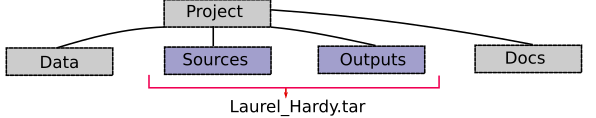
\includegraphics{Figures/architecture.png}
\caption{Exemple de figure: architecture du projet}
\label{fig:2}
\end{center}
\end{figure}

Des figures très soignées ou très jolies impressionnent toujours le lecteur.

Il faut pour cela apprendre à maîtriser les options graphiques des langages comme Matlab ou Python.

 Encore mieux, pour les plus experts, il faut savoir utiliser des logiciels de traitement d'images, comme GIMP par exemple, et des logiciels graphiques vectoriels comme Inkscape. Ces deux logiciels permettent de faire des choses très complexes comme introduire du texte ou des équations dans une figure ou images, ou de superposer des graphes à des images, ou d'autres choses plus complexes. Il faut du temps pour apprendre ces logiciels, mais c'est un investissement rentable pour toute la carrière, en plus des études. 

\subsubsection{Figures en général}

Il existe trois types génériques de figures:
\begin{itemize}
\item des dessins qui illustrent quelque chose, une géométrie, une configuration, une expérience, des mesures,  etc ...
\item des images
\item des graphiques contenant des représentations de résultats numériques sous différentes formes.
\end{itemize}

Parfois une figure est un mélange des trois cas.

Pour tous ces types la figure doit :
\begin{itemize}
\item avoir un numéro  (souvent automatique avec les éditeurs de texte)
\item avoir une légende qui indique clairement le contenu de la figure. La légende peut aller jusqu'à 4 ou 5 lignes parfois, si elle est très descriptive
\item  être centrée sur la largeur de page
\item  avoir une hauteur de 3 à 7 cm. Exceptionnellement elle peut prendre une moitié ou une hauteur totale de page, notamment quand une figure est composé de plusieurs sous-figures.
\item avoir une bonne définition en pixels. Attention aux copies d'écran ou aux images basses définitions qu'on récupère à droite ou à gauche, et qui donne au final un rendu flou
\item respecter le rapport d'aspect de la figure ou image originale. Le rapport d'aspect est le rapport hauteur/largeur. Sinon l'image à l'air d'être étirée dans une direction, ce qui donne un rendu affreux
\item  avoir des  textes  lisible sà l'échelle  100\%, surtout  s'ils sont importants pour comprendre la figure.
\item être positionnée judicieusement dans le document, c'est-à-dire proche de l'endroit où on la décrit. Si ce n'est pas possible, cela indique qu'il n'y a pas assez de commentaires sur les figures et que certaines sont inutiles ou à positionner dans une annexe. 
Deux autres conseils peuvent être donnés:
\begin{itemize}
\item En général on préfère mettre une figure en haut de page ou vers le milieu. 
\item On évite d'avoir une ligne ou deux de texte entre des figures, car en général le lecteur ne les verra pas.
\end{itemize}


\end{itemize}

\subsubsection{Graphiques scientifiques}

Pour les figures représentant des nombres, des fonctions ou  des isolignes ou autre,  il faut veiller à:
\begin{itemize}
\item avoir une légende sur l'axe des abscisses et très très souvent aussi sur l'axe des ordonnées
\item avoir une bonne visibilité des courbes. Cela implique un choix de couleurs, d'épaisseurs ou de taille de symbôles judicieux. 
\item éviter la surcharge de courbe. Au-delà de quelques courbes (3 à 5) on ne voit plus rien sur une figure, sauf si les courbes sont étagées. 
\item avoir une légende pour chaque courbe quand il y en a plusieurs
\item avoir l'échelle des couleurs quand on a des isobarres ou l'échelle des valeurs si possible, quand on a des isolignes.
\item avoir une taille de fonte lisible pour  des nombres et les textes
 sur les axes des abscisses, des ordonnées pour le  titre et les légendes
\item ajouter des lettres lorsqu'on a des sous-figures. Des hauteurs des sous-figures doivent rester décentes (supérieures à 1.5 ou 2 cm). 
\item ce que les échelles sur les deux axes soient choisies judicieusement de manière à ce que le graphique remplisse globalement le cadre. 
\item choisir correctement les axes, en semi log ou log-log ou échelles linéaires
en faisant attention aux signes des valeurs naturellement.
\item  ajouter une grille bien définie si on souhaite prendre des valeurs sur les courbes

\item comparer correctement des résultats lors de validation. On doit avoir par exemple quand c'est possible la courbe résultat et la courbe de référence sur le même graphe, et pas sur deux graphes côte à côte. Lors qu'on est obligé de comparer deux figures côte à côte il faut respecter les dimensions des figures, et avoir des valeurs identiques sur les deux axes, avec une grille.
\end{itemize}

Enfin, quand on fait un commentaire sur une figure, on doit \textbf{faire référence au numéro de la figure}. Le commentaire doit faire quelques lignes. La première chose est de décrire ce qui est représenté. Ensuite on commente les tendances, les variations, les points particuliers (maximun, minimun, discontinuités, ...)

Voici un exemple de commentaire :

La figure \ref{fig:1} représente l'expérience sur un anneau tourbillonnaire (a), un exemple de visualisation à un instant donné(b), et enfin une reconstruction 
de l'anneau tourbillonnaire dans un plan. ... bla bla ...

\bleu{On peut remarque que les nombres sur la figure (c) ont été agrandis et que les épaisseurs des traits sur toutes les figures ont été forcés.}

Deux remarques lorsqu'on veut conserver un graphe pour un rapport ou une présentation:

\begin{itemize}
\item En général dans tous les langages classiques comme Python ou Matlab, les épaisseurs des traits et les hauteurs des nombres par défaut sont optimisées pour la visualisation sur un écran (de grande dimension). Pour une sauvegarde et
une introduction dans un rapport il faut toujours définir les hauteurs et épaisseurs dans le programme et ne pas se contenter des valeurs par défaut. Il faut aussi tenir compte de la possible réduction de l'image dans le document.

\item En toute logique, pour une présentation orale des résultats il faut
refaire des figures spécifiques en augmentant encore la hauteur des textes et l'épaisseur des traits pour améliorer la visibilité via un vidéo-projecteur.
\end{itemize} 

Les figures doivent apparaître dans l'ordre où elles sont nommées. Par exemple ici, je me suis trompé  volontairement en parlant d'abord de la figure \ref{fig:1}
alors que la première à apparaître est la figure \ref{fig:2}.


 
\begin{figure}[htb]
\input{Figures/experiment.pdf_tex}
\caption{Vortex ring experiment and results \cite{Albagnac}, a) experimental set-up,b) example of picture, c) example of the velocity field.}
\label{fig:1}
\end{figure}


 


%**************************
\subsection{Table, tableaux}
%*************************


 
 
 


% Exemple de tableaux





Un  tableau permet de synthétiser des résultats issus de simulations numériques ou des valeurs expérimentales 
ou de fournir des paramètres en un coup d'oeil. 
Il contient donc toujours des informations jugées  essentielles sous la forme de données numériques ou de texte.

\begin{itemize}
\item Il est déconseillé de positionner des tableaux au milieu du texte lorsque cela diminue sa visibilité.
\item Il vaut mieux les insérer comme des figures avec un numéro et une légende.
\item Il ne faut pas oublier de positionner le tableau près de l'endroit où il est évoqué et de le nommer par sa référence
\item Un tableau doit rester sobre.  
 \item On peut ajouter quelques couleurs par alternance, par lignes lorsqu'il y a beaucoup de lignes pour améliorer la lecture
 et minimiser les erreurs de lecture. On peut aussi procéder ainsi pour les colonnes.
\item Préférer un tableau avec des colonnes larges que des colonnes serrées et il faut  centrer le tableau sur la page.
\item le tableau devra être amélioré en ajoutant des couleurs et en augmentant les tailles de fontes 
pour une présentation en mode diapositive
\item s'il y a beaucoup d'information à faire passer, il faut mieux proposer plusieurs tableaux qu'un tableau illisible ou incompréhensible
\end{itemize}




\begin{table}[htb]

\vs{0.5}

\setstretch{1.4}
\small
\centering
\begin{tabular}{p{1.5cm}p{2.5cm}p{2.5cm}p{3.5cm}p{3cm}p{2cm} }
\Xhline{2pt}
Case    &      Fluid    & Velocity     & Reynolds number   &  Flow rate     & Length \\ 
        &               & $U$~[m/s]    & $Re$ in $10^6$  &  $q_m$~[kg/m$^3$] &  $\ell$~[mm] \\ \Xhline{1pt}
1       & Air           & $100$        &   $1.5$         &  $100$            &  $35.33$     \\
2       & Water         &  $\;\;10$        &   $0.1$         &  $\;\;78$             &  $\;\;5.24$  \\
\Xhline{2pt}
\end{tabular}
\caption{Premier exemple  de format de tableau (excellent).}           
\label{tab:exemple1}   
\normalsize
\setstretch{1}
\end{table}


Les tableaux tabs.~\ref{tab:exemple1}, \ref{tab:exemple2} et \ref{tab:exemple3} sont trois exemples qu'on peut rencontrer.

Commentons les.



\begin{enumerate}
\item Le premier tableau tab.~\ref{tab:exemple1} est rencontré dans les publications scientifiques. Il respecte les consignes suivantes:
		\begin{itemize}
		\item Il est sobre avec deux lignes épaisses pour délimiter le tableau dans le plan vertical et une ligne fine
		 qui démarque le titre des colonnes
		 \item Les grandeurs sont clairement décrites avec leur symbôle et leur unités physiques 
		 \item l'interlignage ou espacement vertical est suffisamment important pour améliorer la lisibilité
		 \item les valeurs ou textes sont positionnés à gauche et alignés (on peut aligner sur le . pour les nombres réels)
		 \item le tableau occupe presque la largeur de la page, les colonnes sont dimensionnées précisément.
		 \item le tableau est bien séparé du texte et ressort bien
		 \item on peut remarquer que la hauteur de fonte est légèrement inférieure à celle du texte principale, ce qui peut
		 permettre d'ajouter plus de colonnes et de lignes sans occuper trop de place.
		\end{itemize}
		
		C'est la référence à suivre.
		

		
\item Le second tableau tab.~\ref{tab:exemple1} est aussi acceptable mais souffre de quelques défauts:
		\begin{itemize}
		\item on ne connaît pas le sens des variables
		\item les unités sont répétées inutilement
		\item les colonnes sont trop serrées, elles n'occupent pas l'espace en largeur
		\end{itemize}	
		on peut ajouter qu'il n'y a pas de délimitation horizontale et que l'interlignage est très fort. Mais celà
		n'est pas nécessairement négatif.
		
		On peut alors rajouter le sens des variables dans la légende qu'il faut bien lire pour comprendre le tableau.
		
\begin{table}[htb]
\centering
\setstretch{2}
\begin{tabular}{c|cccc}
Case             & Fluid    & $U$               & $Re$                   &   $q_m$ \\ \hline\hline
1                & Air     & $100$~m/s        &   $1.5 \times 10^6$    &  $100$~kg/m$^3$                       \\
2                & Water   &  $10$~m/s        &   $0.1 \times 10^6$    &   $5$ ~kg/m$^3$      \\
\end{tabular}
\caption{Deuxième exemple de format de tableau (acceptable). La vitesse est notée $U$ et le débit massique $q_m$. }           
\label{tab:exemple2}   
\normalsize
\setstretch{1}
\end{table}
		
\item Le dernier exemple  tab.~\ref{tab:exemple1} est une représentation très basique des données sans aucune réflexion sur le rendu. Ils souffrent de tous les défauts possibles
	   qui sont le contraire des qualités du premier tableau. Il n'est en particulier pas nécessaire de marquer les lignes et
	   les colonnes quand c'est évident. Et il n'y ni unité, ni explication sur le sens des variables. Enfin les lignes et les colonnes sont très resserrées.
	   On peut aussi remarquer que le tableau n'est pas centré sur la page.
	   
	   Cette représentation est à proscrire!
	   
	   
\begin{table}[htb]
\begin{tabular}{|c|c|c|c|c|}
\hline
Case             & Fluid    & $U$          & $Re$                   &   $q_m$ \\ \hline
1                & Air     & $100$        &   $1.5 \times 10^6$    &  $100$    \\ \hline
2                & Water   &  $10$        &   $0.1 \times 10^6$    &   $5$      \\ \hline
\end{tabular}
\caption{Troisième exemple de format de tableau (le plus mauvais) }           
\label{tab:exemple3}   
\normalsize
\setstretch{1}
\end{table}
	   
\end{enumerate}


On peut aussi:

\begin{itemize}
\item ajouter de la couleur soit par ligne, soit par colonne, soit une ligne sur deux et une colonne sur deux pour encore améliorer la visibilité.
\item choisir une couleur unique avec une teinte foncée et claire pour éviter l'effet "arc-en-ciel"
\item encore jouer sur les épaisseurs des traits.
\item modifier les types de fontes par rapport à celle du texte principal pour insister sur le contenu des colonnes
\end{itemize}












 
 

% *******************************************************
\section{Styles spéciaux}
% *******************************************************

En fonction du contexte on peut appliquer des styles spéciaux pour mettre en avant 
des choses importantes. Il faut rester malgré tout sobre.

  

\Attention{Message d'avertissement avec une mention en anglais.}

 
  \Important{Il faut absolument éviter le plus possible les fautes de grammaire et d'orthographe ainsi que les erreurs typographiques.
  
  Pour cela il faut :
  \begin{itemize}
  \item utiliser les dictionnaires intégrés au logiciel de publication
  \item relire le rapport plusieurs fois, en laissant du temps (heures, jours) entre les lectures.
  \end{itemize}
  
  }
  
  


\section{Conclusion}

% ********************************
\chapter{Le contenu}
% *******************************
%% chapter contenu

\section{Introduction}

\section{Contenu technique et scientique}

\section{Valeurs numériques et unités}



On trouve nécessairement des applications numériques ou des nombres ou des valeurs de grandeurs physiques dans un rapport de TP :

\begin{itemize}
\item Toute valeur numérique qui a un sens physique doit  nécessairement être
 accompagnée de son unité.
\item Suivant les problèmes on donne entre 3 et 5 chiffres significatifs et donc il faut utiliser judicieusement les puissances de 10.
\end{itemize} 

\section{Apport personnel}


\section{Conclusion}

%*********************************
\chapter{Conclusions, perspectives}
%*********************************
%% Conclusion et perspectives



Tout corps de rapport doit se terminer par une section ou un chapitre "conclusions 
et perspectives". 

Il est courant que le lecteur commence même par lire ce chapitre avant tout le reste pour directement évaluer l'intérêt de regarder plus ou pas, c'est donc une partie à particulièrement soigner.

%********************
\section{Conclusions}
%********************

Dans cette rubrique on doit trouver les conclusions scientifiques ou techniques, qui sont étayées par les résultats obtenus. 

Il faut rappeler les objectifs du projet, et en quelques lignes les méthodologies employées. 

Il faut ensuite rappeler les principaux résultats et les conclusions qu'on en tire. Il faut parler de fait, et éviter les supputations.

Enfin il faut insister sur les aspects originaux du travail et son apport personnel\footnote{On utilisera le passif ou le "on". Il faut éviter le "je" car il est très rare que vous ayez fait le travail tout seul, sans aucune aide extérieure.}

%*********************
\section{Perspectives}
%*********************
 
Il faut démarrer sur des perspectives directes, à courte échéance, qui correspondent à une suite directe du travail accompli.

Ensuite on peut laisser plus de place à l'imagination en donnant des perspectives plus lointaines, mais réalistes. Cela peut devenir de nouvelles orientations du projet en cours.

Les perspectives sont souvent les parties les plus lues en détail car c'est l'aboutissement du travail et une potentielles sources d'inspiration pour continuer le projet.

% *********************************
\section{Conclusions personnelles}
% **********************************

Cette section n'est à mettre que pour un rapport de stage ou de projet
et uniquement à destination des universitaires.

Dans les rapports d'entreprise on n'a pas ce genre de section, sauf si cela
est demandé explicitement.

Il faut rester assez neutre, en rappelant les côtés positifs du stage, tout en 
énonçant les difficultés rencontrées, et en indiquant finalement 
ce qui a été appris, et les nouvelles compétences acquises.



%***********************************
\section{**Conclusion, perspectives}
% **********************************

Quelque soit la rédaction, un document contient nécessairement une introduction et une conclusion.

Pour un compte-rendu, cela est l'occasion de rappeler l'intérêt du TP, ce qu'on a pu apprendre, les difficultés rencontrées et donner par exemple son avis personnel.

On peut ajouter des perspectives.

Pour un compt-rendu,   10 à 15 lignes suffisent amplement.


\vspace{1cm} 
 
La qualité du rapport démontre votre investissement. Un étudiant qui n'a rien compris ou rien fait en TP ne pourra jamais faire un bon rapport. 
Un beau et bon rapport mettra en valeur vos compétences, vos connaissances 
et votre capacité de travail et de compréhension. 
 
\Important{Enfin tout rapport doit contenir une bibliographie, avec des références contenant toutes les informations pour retrouver le document, comme ce qui est fait dans l'exemple ci-dessous.
Cela peut être juste le cours du professeur ou un livre.}


% une façon de faire apparaitre toute la bibliographie
\cite{*}

% on finit par une ligne horizontale pour indiquer que c'est la fin ... (optionnel)
\hrule height 0.5 mm 

\vs{0.5}

% ajout de la bibliographie (obligatoire)

\addcontentsline{toc}{chapter}{Bibliographie}
\markboth{{Bibliography}}{}
\markright{{Bibliography}}{}
\bibliography{biblio_reporting}

% Ajout des annexes (optionnel)
%*********************************
\chapter{Annexes}
%*********************************
%% Annexes


%*****************
\section{Annexes}
%****************

On peut ajouter une ou deux pages d'annexe. Le format est plus libre car
l'annexe n'est pas toujours lu. On peut avoir par exemple uniquement des figures, ou des équations avec très peu de commentaire.

\subsection{\'Equations du problème}

\vspace{2cm}

\subsection{Figures supplémentaires} 

\vspace{2cm}

\end{document}

% Tout ce qui est écrit après end{document} ne sera pas pris en compte.

